\documentclass[12pt, letterpaper]{article}
\usepackage[english]{babel}
\usepackage{adjustbox}
\usepackage[utf8]{inputenc}  
\usepackage{csquotes}
\usepackage[authordate,backend=biber]{biblatex-chicago}
\usepackage[margin=1in]{geometry}
\usepackage{abstract, multirow, pdflscape, floatrow, parskip, fancyhdr, amsmath, tabularx, tabu, titlesec}
\usepackage{float, array, indentfirst, amssymb, titlesec, hyperref, longtable, listings}
\usepackage[format=plain,up,textfont=normal,up,justification=justified,singlelinecheck=false]{caption} 
\usepackage[bottom,flushmargin,hang]{footmisc}
\usepackage{amsmath}
\usepackage{pgfplots}
\pgfplotsset{compat = newest}
\usepackage{abstract, amsmath, amssymb, array, indentfirst, fancyhdr, floatrow, listings, longtable, multirow, biblatex, pdflscape, setspace, tabu, tabularx, titlesec, url}
\usepackage{booktabs,wrapfig}
\usepackage{siunitx}
\newcolumntype{d}{S[
	input-open-uncertainty=,
	input-close-uncertainty=,
	parse-numbers = false,
	table-align-text-pre=false,
	table-align-text-post=false
	]}
\usepackage{tikz}
\newcommand*\circled[1]{\tikz[baseline=(char.base)]{
		\node[shape=circle,draw,inner sep=2pt] (char) {#1};}}
\usepackage{fancyhdr} 
%\usepackage[justification=centering]{caption}
\usepackage[final]{pdfpages}
\usepackage{floatrow}
\captionsetup[table]{singlelinecheck=false,justification=centering,position=bottom}
\captionsetup[figure]{singlelinecheck=false,justification=centering,position=bottom}
\hypersetup{colorlinks=false,
	pdfborder={0 0 0},}
\setlength{\parindent}{24pt}
\newcommand{\forceindent}{\leavevmode{\parindent=2em\indent}}
\pagestyle{fancy}
\lstset{basicstyle=\ttfamily, columns=flexible, breaklines=true}
\fancyhf{}

\lhead{\footnotesize{Smart Student \\ Research Note 1}}
\rhead{\footnotesize{GVPT999 \\ \today}}

\renewcommand{\arraystretch}{1.2}

\renewcommand{\headrulewidth}{1pt}
\fancyfoot[C]{\footnotesize\thepage}
\newcolumntype{R}{>{\raggedright\arraybackslash}X}
\titleformat{\title}{\section}{\large\bfseries}{\thesection}{1em}{}
\setlength{\parskip}{0pt}
\doublespacing

%\addbibresource{rn.bib}

\begin{document}
	
\setlength{\parindent}{1cm}
\parskip=0pt

\subsection*{\centering Title}

\noindent XXX

\pagebreak

\begin{table}
	\centering
	\caption{Mean predicted probabilities}\label{t2}
	\begin{tabular}[htpb!]{lc}
		\hline\hline
		& Mean \\ 
		\hline
		Model 1: Mean Difference & -0.074 \\ 
		Model 1: Mean Sim. Difference & -0.066 \\ 
		Model 2: Mean Difference & -0.137 \\ 
		Model 2: Mean Sim. Difference & -0.123 \\ 
		\hline
	\end{tabular}
\end{table}

\begin{figure}[t!]
	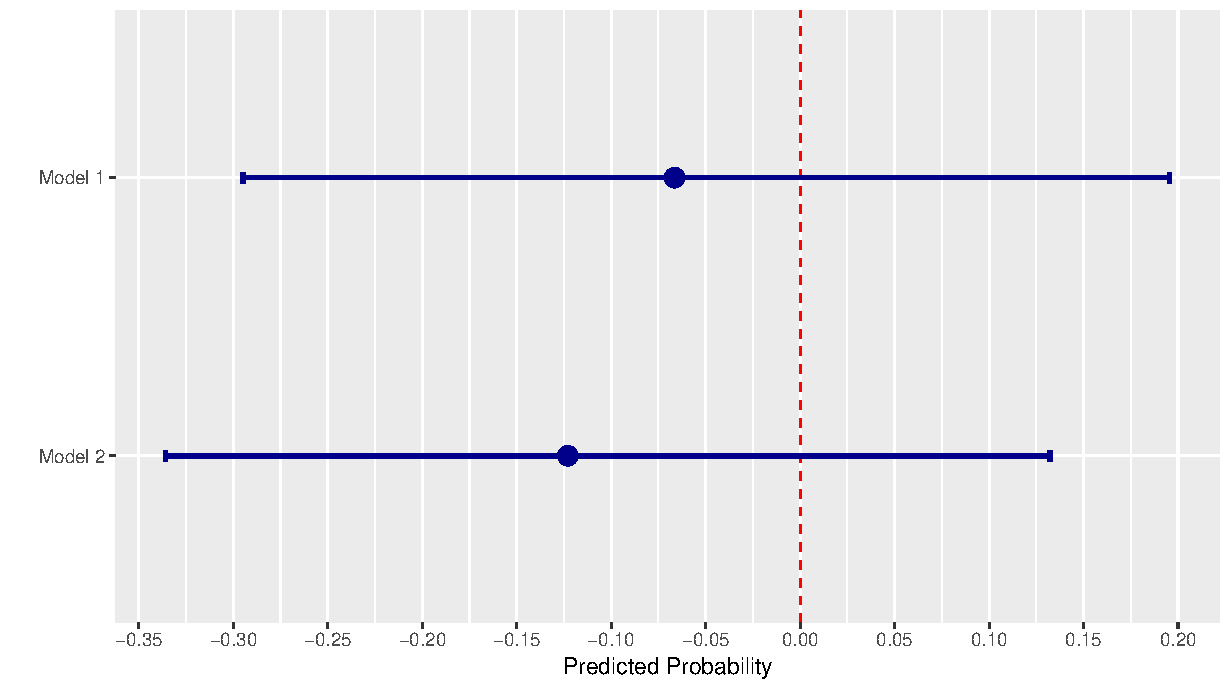
\includegraphics[scale=.7]{predplot.pdf}
	\caption{Mean simulated predicted probabilities and 95\% CIs}\label{f1}
\end{figure}

%\clearpage

%\pagebreak
%\singlespacing
%\begingroup
%\titleformat*{\section}{\fontsize{14pt}{18pt}\bfseries\selectfont}
%\printbibliography
%\endgroup

\end{document}